\section{Resisitive switch design}
\label{sec:resisitive_switch_design}
- Mechanical concept: Simple beam, contact pad, actuation pad
- Simplifications

\subsection{Basic concepts}
\label{sec:basic_concepts}
Area moment of inertia of recangular section:
\begin{equation}
	I_z = \frac{bh^3}{12}
	\label{eq:area_moment_of_inertia}
\end{equation}

Deflection of a beam:
\begin{figure}[h]
	\centering
	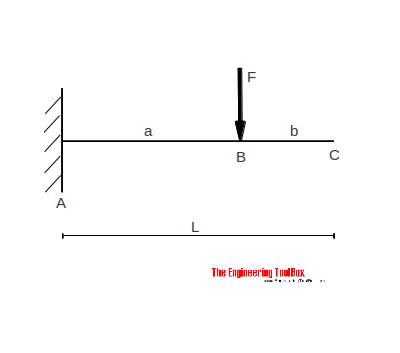
\includegraphics[width=8cm]{fig/cantilever_beam_single_load.png}
	\label{fig:cantilever_beam_single_load}
\end{figure}

\begin{equation}
	\delta = \frac{F}{3EI}\cdot\frac{a^3(1+3b)}{2a}
	\label{eq:beam_deflection}
\end{equation}

- Frequency response / Minimal switching
Spring constant:
\begin{equation}
	k = \frac{F}{\delta} = \frac{Ewt^3}{4L^3}
	\label{eq:spring_constant}
\end{equation}

Resonance frequency:
\begin{equation}
	\omega_0 = \sqrt{\frac{k}{m}}
	\label{eq:resonance_frequency}
\end{equation}


- Electrostatic analysis
- Failure

\subsection{Analysis}
\label{sec:analysis}
- Actuation point vs contact point placement
- Area contact
- Area actuator
- Beam cross section
- Material
